\section{Figure Rendering}

\subsection{3D Plots}

\begin{figure}[h]
    \centering
    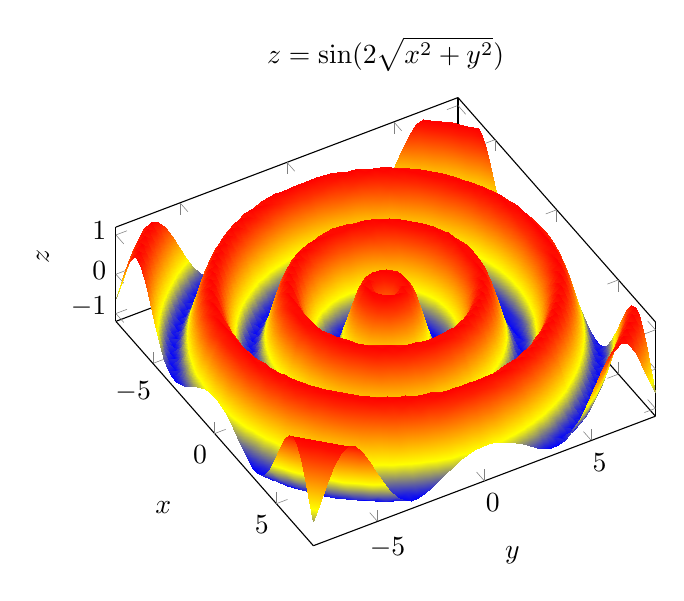
\begin{tikzpicture}
    \begin{axis}[
        title={$z = \sin(2\sqrt{x^2 + y^2})$},
        xlabel={$x$},
        ylabel={$y$},
        zlabel={$z$},
        domain=-8:8,
        y domain=-8:8,
        view={60}{70},
        samples=50
    ]
    \addplot3[
        surf,
        shader=interp,
    ]
    {sin(deg(2*sqrt(x^2 + y^2)))};
    \end{axis}
    \end{tikzpicture}
    \caption{3D plot of $z = \sin(2\sqrt{x^2 + y^2})$}
\end{figure}

\subsection{Circuit}

\begin{figure}[h]
    \centering
    \begin{circuitikz}[american voltages]
        \draw
          (0,0) to [short, *-] (6,0)
          to [V, l_=$\mathrm{j}{\omega}_m \underline{\psi}^s_R$] (6,2) 
          to [R, l_=$R_R$] (6,4) 
          to [short, i_=$\underline{i}^s_R$] (5,4) 
          (0,0) to [open, v^>=$\underline{u}^s_s$] (0,4) 
          to [short, *- ,i=$\underline{i}^s_s$] (1,4) 
          to [R, l=$R_s$] (3,4)
          to [L, l=$L_{\sigma}$] (5,4) 
          to [short, i_=$\underline{i}^s_M$] (5,3) 
          to [L, l_=$L_M$] (5,0); 
        \end{circuitikz}
    
    % Caption and label for the figure
    \caption{Random Circuit} 
    \label{fig:my_label}
\end{figure}